This chapter presents our approach for answering the research questions mentioned in Chapter~\ref{chapter:introduction}. Before diving into the details of our methods, in Section~\ref{section:scenario}, we first introduce a concrete scenario motivating the research questions: A translation company wants to improve the quality of NMT systems by only using fragmented data instead of full sentences as a compromise.
%In addition, Section \ref{section:threat_model} makes a explicit threat model that we want to prevent. 
Based on the scenario, we finally propose our solution for the given problem. Our approach consists of two parts: Extraction of fragment text and domain adaptation for NMT. In Section \ref{section:phrase_pairs}, we propose to use \textit{phrase pairs} as a parallel corpus fragmentation method. %Then, we use domain adaptation with phrase pairs of in-domain dataset.
In Section \ref{section:domain_adaptation_nmt}, we suggest domain adaptation of a NMT model with phrase pairs. Specifically, we choose fine-tuning, the most conventional way for domain adaptation in NMT. Finally, in Section \ref{section:pipeline}, we present the pipeline to implement and evaluate the proposed method based on the motivated scenario. 

%but this can cause overfitting. To prevent that, we also use several regularization techniques and this will be covered in Section~\ref{section:Regularization}.
%We show our motivating scenario where a translation company provides deep learning based customised translation services to the different clients, and this company pursues the better translation quality when there is not enough in-domain. Based on the scenario, we introduce our method.\SK{should change this sentence later :(} We explain the phrases used as a method of fragment parallel corpus and how it was used. After that, we cover domain adaptation for machine translation.
%In this project, we will explore the possibility of using otherwise unavailable confidential data to improve NMT models
%%%%%%%%%%%%%%%%%%%%%%%%%%%%%%

%explain what is post-editing
\section{Scenario}\label{section:scenario}

%Nevertheless, the quality of the NMT system is lower than that of human translation, therefore, NMT-based services are suitable for situations different from human translation. They are mainly aimed at clients with the following needs: Clients need to translate large volumes of text on a regular basis in the same language combinations in a particular industry, and only need rapid and adequate translations. 

The translation industry has long been limited to human translation, but as the performance of MT models has improved in recent years, the use of MT is increasing to reduce costs and increase productivity. For instance, a law firm that operates across countries often needs to translate day-to-day manifold documents written in foreign languages. In this case, using only human translation is too expensive and time-consuming, therefore, MT based services are appropriate.
In the early days, Statistical Machine Translation (SMT) dominated commercial MT systems, but by around 2016, many companies have started using deep learning approaches for production systems, such as \textsc{Google Translate} \parencite[]{zhang-etal-2019-bridging}, and \textsc{DeepL}. In this thesis, we focus on translation service based on the NMT pipeline, thus MT service denotes NMT. 

% MT services and domain adaptation
Many MT-based translation companies apply various solutions to improve translation quality. The most widely used method is customising their models to the customer's domain because the general NMT performs poorly for domain-specific translations. %In fact, the text that needs to be translated is often domain-specific fashion, especially if professional or business translation is required.
In the aforementioned example, the law firm wants to translate the documents, which is often the legal domain, and using a generic NMT system can result in the loss of subtle nuances or terminology of the text. For instance, ''stay'' means ''remain'' in general context but in legal domain, it often refers to the postponement or suspension of a judicial proceeding~\parencite[]{Encyclopedia}. When the NMT system is trained on data that is relevant to the organisation's domain, the ambiguous word problem can be lifted. As a result, many translation enterprises offer a custom MT system that uses supervised domain adaptation. 

%Post-editing
Although NMT systems show the state-of-art translation quality, it is still inferior to human translation quality~\parencite{laubli-etal-2018-machine}. To ensure official translation quality, MT companies provide NMT solutions with post-editing that indicates correcting grammar and spelling errors to improve the translation quality by human translators. If necessary, professional translators not only correct errors but also rewrite the text to meet the level of manual translation. %Although post-editing requires more cost and time than only MT solution,
Post-editing with NMT systems benefits cost savings, shorter lead times and reduced cognitive effort compared to manual translation, especially, domain-specific translation
~\parencite{daems2017translation, jia2019does, laubli-etal-2019-post, toral2018post}. 
%post-editing the translation produced by the PBMT results in 594 words per hour, an 18% increase in productivity, while post-editing the NMT output leads to double that figure: 36% (685 words per hour). This is clearly indicative of the fact that NMT outputs were superior to those from PBMT. time savings doubled with NMT (+36%) compared to SMT (+18%) in literary translation (Toral et al., 2018b).
%but post-editing domain-specific texts reported to be faster than from-scratch translation~\parencite[]{daems2017translation}. 
%In addition, clients want not only the better translation quality but also confidentiality protection of their texts. They are concerned about the exposure of information that should not be leaked while using MT engines.
%Many companies provide translation services based on MT systems, from public general MT services such as \textsc {Google Translate} to professional MT services.
%In particular, the professional MT services is suitable in different contexts, mainly providing content for improvement by human translators.
%There are free public MT services such as \textsc{Google Translate} but, for business or professional use, there exist many companies that provide a translation service based on using customised MT engines to clients. 

\subsection{Proposed scenario and solution}

\begin{figure}[!htb]
    \centering
    \hspace{-3mm}
    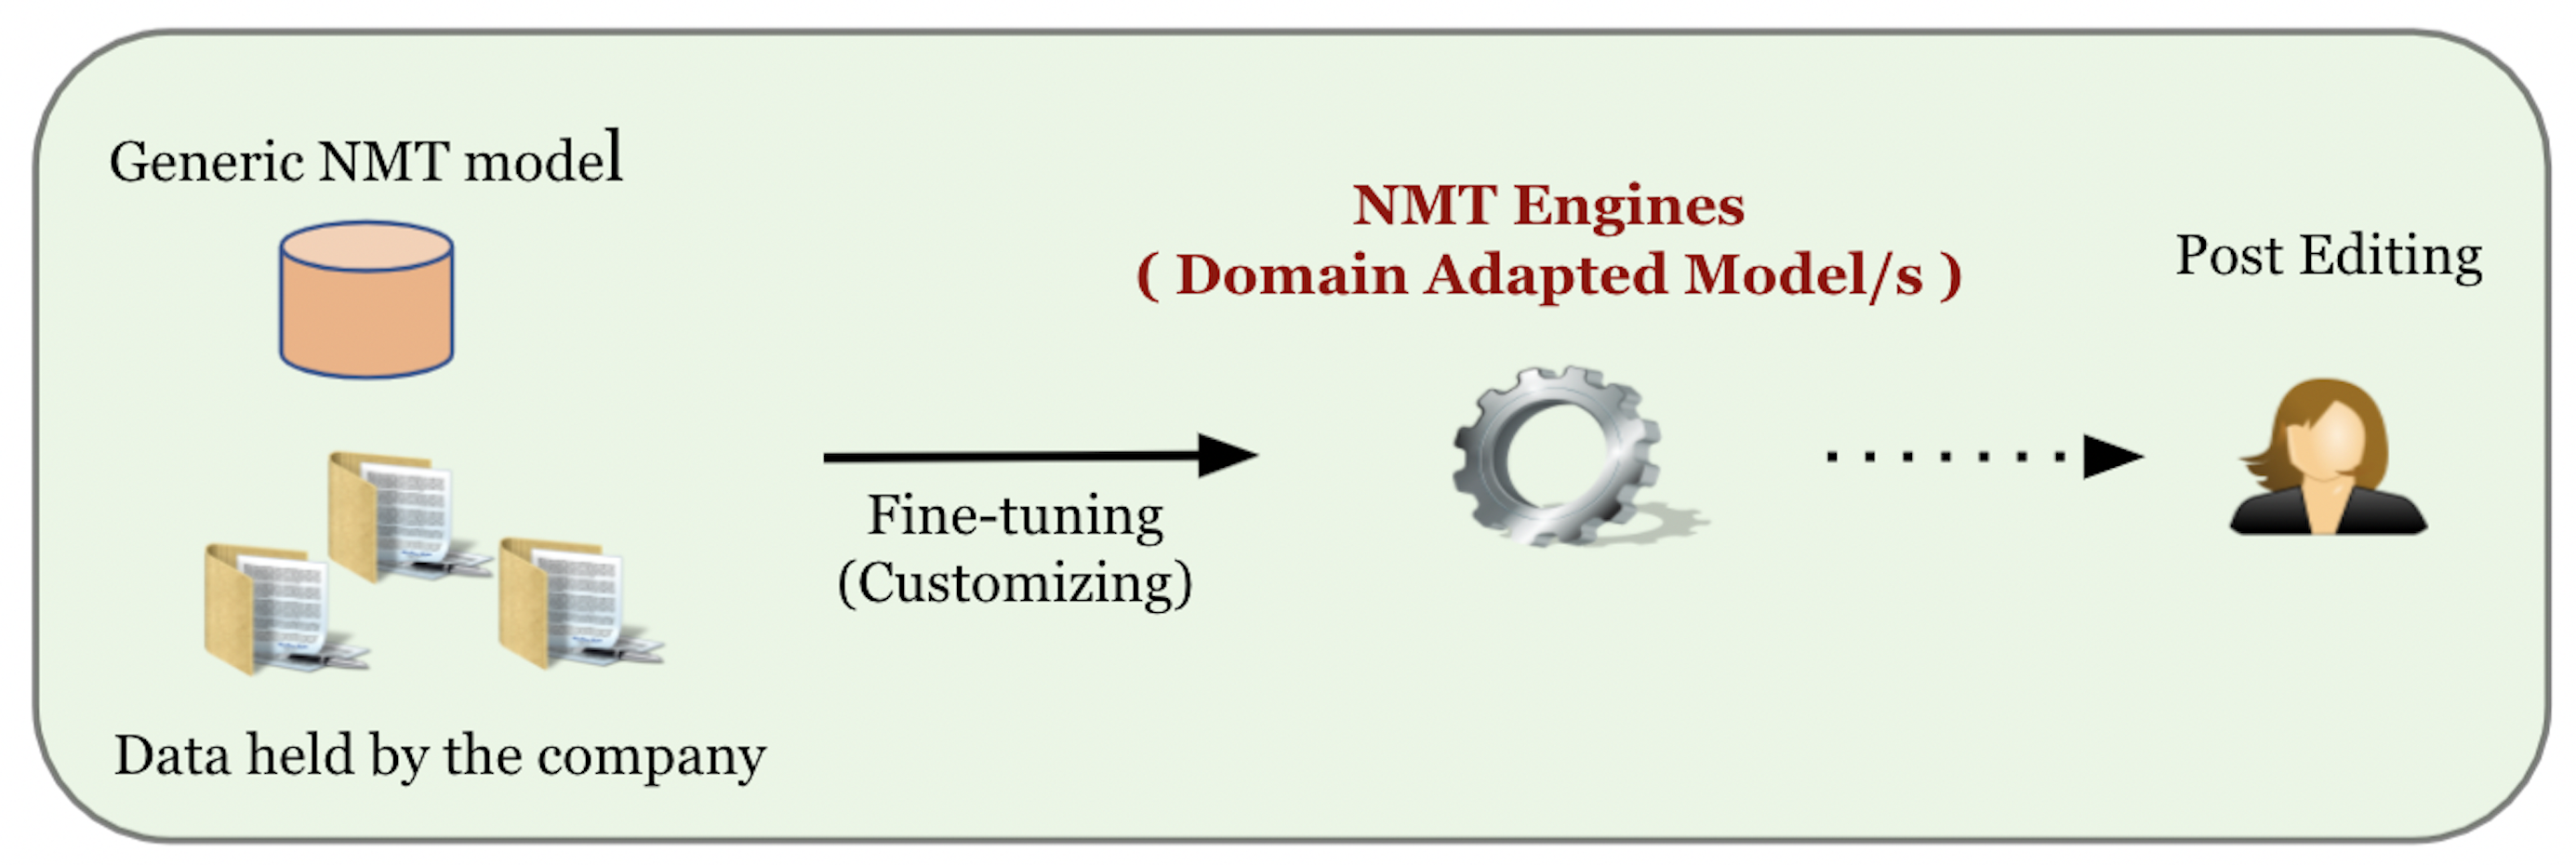
\includegraphics[scale=0.28]{images/companyA.png}
    \caption{ The overview of the pipeline translation company \textit{\textbf{A}}.}
    \label{fig:companyA}
\end{figure}
\begin{figure}[!htb]
    \centering
    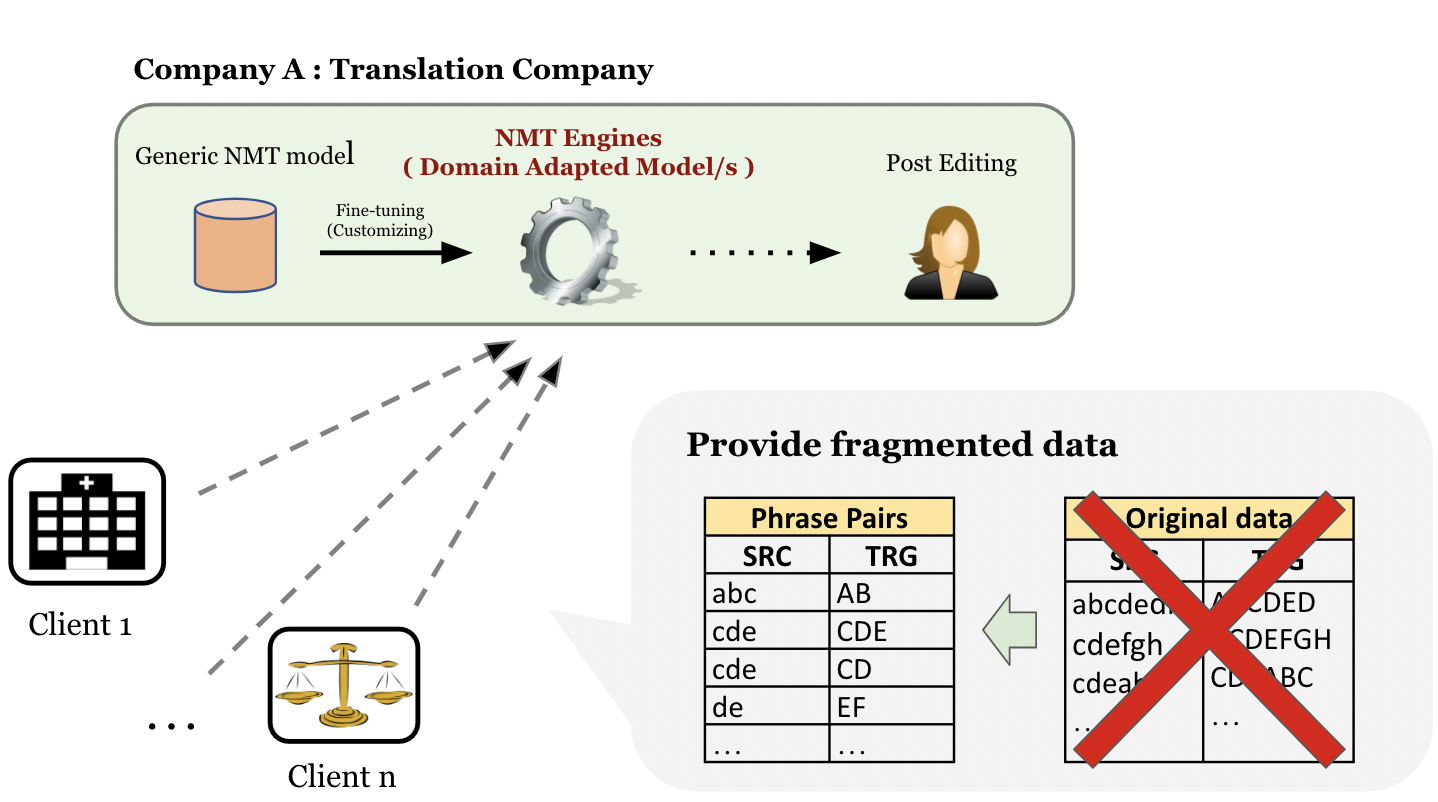
\includegraphics[scale=0.57]{images/motivated_scenario.png}
    \caption{ Proposal scenario : a Translation Company (\textit{\textbf{A}}) uses fragmented confidential data from its clients to adapt a pre-trained generic NMT system to different industry (e.g. medical, legal) domains. }
    \label{fig:scenario}
\end{figure}

To clarify the motivation of our study, we consider a common case where a translation company called \textit{\textbf{A}} provides professional translation services by using an NMT solution. As Figure~\ref{fig:companyA} illustrates, its pipeline consists of NMT system and human post-editing. Company \textit{\textbf{A}} customises the generic NMT model into multiple industry domains for each client to ensure the high NMT quality. To do this, each domain-specific data held by \textit{\textbf{A}} is used for domain adaption. Then, specialised human translators refine the output of NMT engines as a post-editing step. Although \textit{\textbf{A}} has many domain-specific datasets by itself, there may be limitations to using only them to reflect every clients' domains. It is likely difficult to apply more granular domains to an NMT system, or certain terminology frequently used by clients can not be handled properly, which increases post-editing costs and times. 

As a solution, \textit{\textbf{A}} wants to improve the quality of its NMT models by training or adapting them on the clients' previously translated documents. However, due to confidentiality and privacy concerns, the clients do not often share the original documents and its translation to \textit{\textbf{A}}. Instead of sharing the full text, as illustrated in Figure~\ref{fig:scenario}, we consider a scenario that clients of \textit{\textbf{A}} provide their data and translation only in a fragmented form as a compromise for fine-tuning generic NMT system. If this kind of data can be used to improve the NMT model, both the clients and the company will benefit by abating human post-editing costs and turnaround times. Thus, we want to study the possibility of sharing fragmented data for improving utility while preserving the confidentiality of data. 

We propose using \textit{phrase pairs} as a text fragment method. In our proposed scenario, the full sentences of the original documents are not allowed for Company \textit{\textbf{A}} and only extracted phrases are shareable. Therefore, we use the phrase pairs as parallel in-domain data for fine-tuning a baseline model. In addition, we assume that \textit{\textbf{A}} already owns a high-performance generic NMT system, therefore, we choose a strong out-domain pre-trained NMT model. 
%Lastly, we suppose such confidential data that can be released in the fragmented format may consist of a small number of sentences. Therefore, we reserve a relatively small size of data. 


\subsection{Threat model}\label{section:threat_model}
%Key words : confidential information, not user-specific information
%Loss of corporate information such as trade secrets, sensitive corporate information, and details of contracts, or of government information is frequently unreported, as there is no compelling reason to do so in the absence of potential damage to private citizens, and the publicity around such an event may be more damaging than the loss of the data itself
%An honest but secure (HBC) protocol is a secure protocol where attackers are restricted to following the protocol, but after the experiment is over, they may analyse the data they have received to try to recover other players’ inputs. Once they have done so, they may return a result deviating from the regular computation.

In this section, we detail the threat model that is used in this study to define properly the attacker’s goal. % or privacy considerations. 
We assume an \textit{honest but curious} model in which the receiver of the partial data (e.g. the translation company) is not trusted or only partially trusted by the data owner. Honest but curious setting implies the adversary follows the rules but can later infer the information of the rules for malicious purposes~\parencite{goldreich2009foundations}. The main threat we focus on is the \textbf{full reconstruction} of the original text from a list of given n-grams of phrases rather than the protection of partial information (e.g. key phrases~\parencite{hard2018federated}, names, social security numbers). Thus, the confidentiality consideration in our study is that 'secrets' of clients may leak when a NMT model is fine-tuned on confidential data that contains sensitive business information. The secrets stand for the core information from which the data owners obtain financial benefits. This setting is useful in various contexts where only partial data release is desired such as copyright protection. Examples of text where sensitive information is encoded in long sequences (sentences or paragraphs) include patent applications, as well as not (yet) publicly available product analysis reports, drug reaction reports or technological processes of software. Our study is the first step in opening the possibility of using compromised fragmented data for NMT when the original data is unavailable.

%However, the motivation that confidentiality is improved by releasing partial sequences, or that confidentiality is compromised by releasing complete sequences, is not motivated: no examples are shown to illustrate how sequences contain confidential information, nor how that confidentiality is preserved after applying the method, nor are specific threats to confidentiality enumerated. This concerns the missing threat model: how would an attacker attack the sequence data to compromise confidentiality, and how would this approach reduce the attack surface?

\section{Phrase Pairs}\label{section:phrase_pairs}
% why phrase pairs ? 
% and what is phrase pairs?
% what we can expect from fine-tuning NMT on phrase pairs?
% how to present phrase pairs will be covered in experimental section ( fine-tuning )
In the previous section, we presented a solution in which only fragments of the original data are used for domain adaptation of the NMT system. In NLP, releasing fragmented data in the form of N-grams has a long tradition such as Google N-grams~\parencite{michel2011quantitative}. This corpus provides insight into annual trends through N-grams and statistics, but restricts access to specific subsets of documents. However, fixed-size N-gram extraction is not directly applicable to parallel data because it breaks translation equivalence with the target side. As a solution, we propose to use \textit{phrase pairs} as a text fragmentation method.

Like N-grams, phrases are short sequences of consecutive words extracted from the input sentences. Unlike N-grams, phrases are always extracted in pairs from source-target sentence pairs in a way that is \textit{consistent} with their word-level alignment. Formally, a phrase pair $(\bar{f}, \bar{e})$ is consistent with word alignment $A$ if all source words $f_1, \cdots, f_n$ in $\bar{f}$ that have alignment points in $A$ are connected with target words $e_1, \cdots, e_m$ in $\bar{e}$ and vice versa \parencite{koehn2003statistical, koehn_2009}. 
As Figure~\ref{fig:example_phrase} illustrates, the words of the target language (German) are first automatically aligned (grey connecting lines) with the words of the source language (English) by a statistical alignment model. Then, phrase pairs of various lengths (denoted by boxes) are extracted. A user can limit the maximum length of the phrases. This example is extracted with maximum length 3 that denotes the source side phrases must consist of up to 3 words. 

%How the phrase is extracted is based on the alignment between these source and target words. However, the statistical alignment model creates many-to-one word alignment to target language and it can cause error alignments eventually.
% As a solution, use alignments in both directions and combine them with various heuristics to grow intersection\cite{koehn2003statistical}. 
\begin{figure}[hb!]
    \centering
    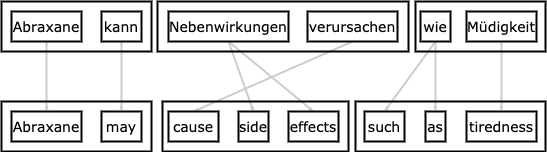
\includegraphics[scale=0.63]{images/phrase_example.png}
    \caption{Sample of extracted phrases from EMEA training dataset.}
    \label{fig:example_phrase}
\end{figure}

Phrase pairs and their statistics constitute the main component of Phrase-based SMT (PB-SMT) systems, together with the target language model.
%the phrases are statistically translated into target language and reordered. 
In this work, however, we only use phrase extraction as a text fragmentation technique.

\subsection{Preserving Confidentiality}

We aim to ensure that the attacker cannot reconstruct the entire original document from the extracted phrases.
After extraction, we shuffle the large set of phrase pairs extracted from the whole dataset and, finally, discard a random sample of phrase pairs (e.g. 50\%) to preserve confidentiality. 
In the example of Figure~\ref{fig:example_phrase}, this would mean protecting the hypothetically sensitive connection between the drug name (\textit{Abraxane}) and its reported side effect (\textit{tiredness}). 

%%%%%%%%%
%We use \textit{phrases} as a text fragmentation method which ensures data confidentiality while leaving the sentence alignment valid. Phrases are basically groups of words that are segmented from the input sentences. Phrase pairs are extracted using heuristic word-to-word alignment. As Figure \ref{fig:example_phrase} illustrates, the words of the target language(German) are aligned with the words of the source language(English). Based on this, the phrases are statistically translated into target language and reordered. In this paper we will often mention using only phrases smaller than a certain length, here we only restrict the target phrase length. For instance, in Figure \ref{fig:example_phrase}, the green boxes represent a phrase of length two: 'der Nachrichtenlist' is the German phrase and 'the list of messages' is the English phrase. In our experiments, the goal is to find the optimal way in which to represent the extracted phrases to pre-trained NMT model.


%%%%%%%%%%%%%%%%%%%%%%%%%%
\section{Domain Adaptation}\label{section:domain_adaptation_nmt}

%Many words have daily-life meanings, but as domain-specific terms they often do not need to be translated.
In our solution, phrase pairs are proposed as a compromise instead of using whole sentences to improve the NMT system. However, fragmented text such as phrases is not an appropriate form to train NMT systems. Phrase pairs are the main components for training most SMT models rather than whole sentences. SMT models obtain informative statistics from phrase pairs for translation. However, due to encoder-decoder architecture~(Section \ref{section:NMT}), NMT models expect full sentences as input, which allows them to better exploit larger context. Indeed, this is one of the main strengths of NMT over the traditional SMT approach.
As a result, training NMT on such fragmented data is likely to lead to very poor performance as a significant amount of contextual information is lost. Nonetheless, we postulate that phrase pairs may still contain very valuable information for the \textit{adaptation} of a general-domain system to a specific target domain. In fact, much of domain adaptation has to do with learning new words or short phrases, as well as new senses for known words and phrases \parencite{irvine-etal-2013-measuring}. 
%Note that, in our study, domain refers to 'topic', such as financial or life-science.

\begin{figure}[ht!]
    \centering
    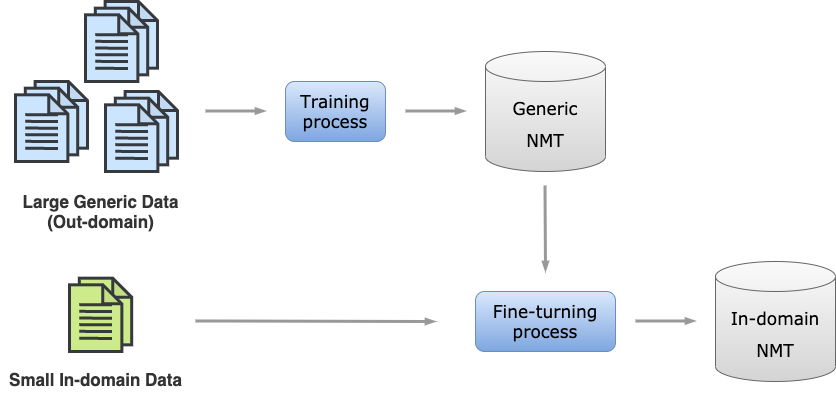
\includegraphics[scale=0.45]{images/domain_adaptation_nmt.png}
    \caption{Fine-tuning for neural machine translation. }
    \label{fig:fine_tuning}
\end{figure}

%There are varying methods for domain adaption for NMT, and a comprehensive review of the possible techniques are introduced by \cite[]{chu-wang-2018-survey}. This can be categorised into two groups as Figure~\ref{fig:domain_adaptation_chart} represents. 
%Since the phrase pairs we use in this study are parallel data, this belongs to the model-centric category. 
Our motivation for this study is to assess the possibility of using fragmented data without changing the architecture of a NMT system, thus we choose \textit{fine-tuning} as the domain adaptation technique. Fine-tuning is a simple but effective strategy for domain adaptation of NMT and is currently considered the most conventional method~\parencite{luong2015stanford, sennrich-etal-2016-improving}. 
As Figure~\ref{fig:fine_tuning} describes, in the fine-tuning process, an NMT model, which is pre-trained on large out-domain data, continues to train on small in-domain data until the convergence.
We start by directly fine-tuning a general-domain NMT system on a random sample of phrase pairs (occurrences, not types) extracted from the in-domain dataset.

\section{Tagging}\label{section:tagging}
%It is expected to bias the phrase adapted NMT model to produce shorter sentence than fine-tuning on whole sentences. As a solution, we experiment with a simple phrase tagging technique \parencite{sennrich2016controlling} so that the model may learn to represent the special nature of phrases and be less inclined to produce short outputs when translating full sentences in the test phase. 
%Re-motivation the length is an important factor to mention. Also explain how and why tagging was used in previous work

%raise problem - short output bias 
In our solution, we present phrase pairs as input for the fine-tuning process of an NMT system. However, these samples are much shorter than the full sentences that were used for the pre-training process of the NMT model. This can cause phrase-adapted NMT systems to have a bias in producing relatively shorter translation outputs compared to fine-tuning on whole sentences. When the output is shorter than the reference, this is affected in lower evaluation. For instance, BLEU (Section~\ref{section:evaluation_metrics}) applies a brevity penalty to short translations compared to references.
To prevent this bias, a fine-tuned NMT system on phrase pairs should be able to recognise the difference between phrases and whole sentences. This way, even when the model is fine-tuned on phrases, it may produce outputs of normal length when translating entire sentences.
%This way, even when the model is fine-tuned for the syntax, it can produce output of normal length when translating the entire sentence.

To teach the NMT model the difference between phrases and whole sentences during fine-tuning, we use a simple tagging technique inspired by~\cite{sennrich2016controlling}. 
The paper shows that adding artificial tags on source sentences of training data to encodes the use of politeness can control the politeness in target side at testing.
Additional tags on either the source or target side help NMT systems to distinguish specific features of the data during training and finally improve translation quality at test time. %Since NMT models have encoder-decoder architecture, they can pay attention to the feature of data.
This is a very effective and simple solution that does not require any changes to the architecture or other parameters.
Recently, the tagging technique has also been used to differentiate various features such as multi-domains~\parencite{kobus-etal-2017-domain}, gender~\parencite{kuczmarski2018gender} and different languages~\parencite{johnson-etal-2017-googles}. In our work, by appending tags to each phrase while fine-tuning, we provide the NMT system with information that phrases are a different type of input than normal sentences.


% we additionally append a tag in front on every sentence while training to indicate the origin data set of each sentence
% the model differentiate between the data.
% The attentional encoder-decoder framework is then able to learn to pay attention to the side constraints.
% The additional token method consists of adding an artificial token at the end of each source sentence to let the network pay attention to the domain of each sentence pair.
% For instance, consider the next English- French translation:
% More recently, Caswell et al. (2019) empirically demonstrated  that  adding  a  unique  token  at  the beginning of each back-translation acts as a tag that helps the system during training to differentiate back-translated data from the original parallel training data
%We experiment with a simple tagging technique by adding <PT> and </PT> at the front and end of each phrase respectively, in both source and target side. During testing, full sentences with no tags are given to the model.

\section{Pipeline}\label{section:pipeline}

\begin{figure}[h]
    \centering
    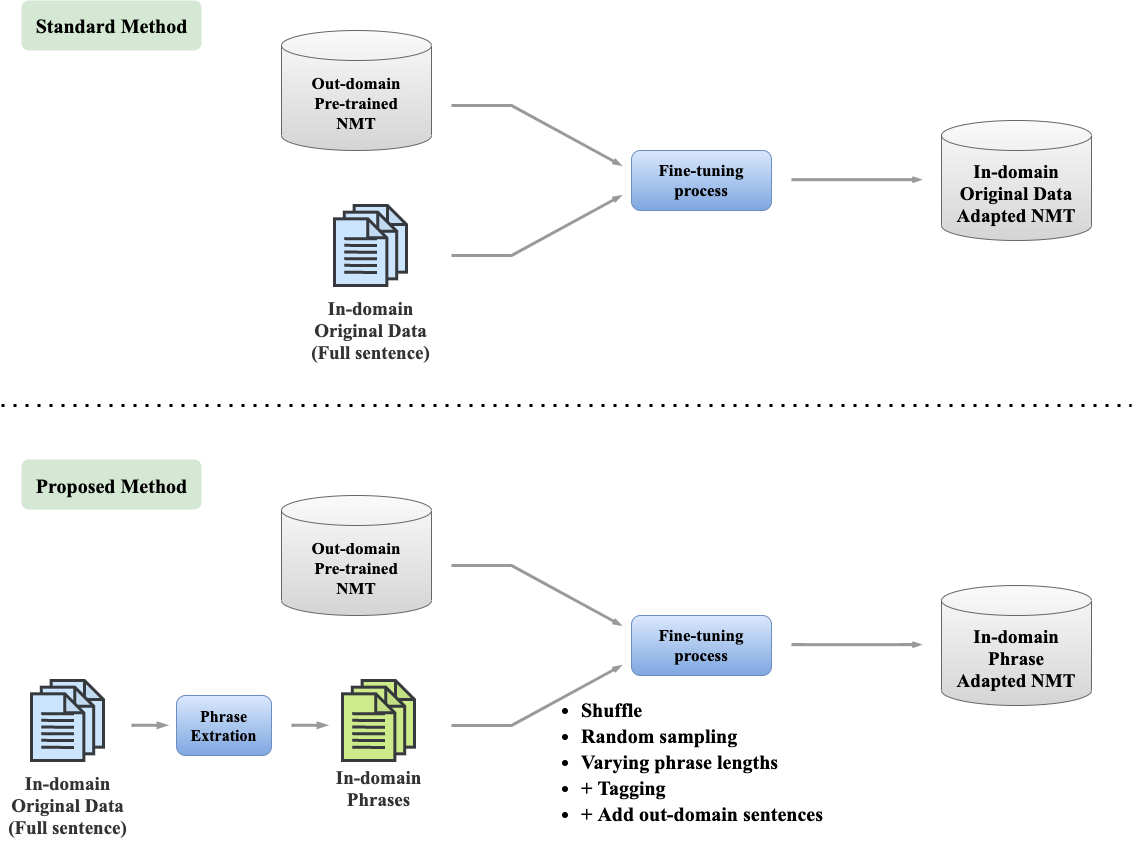
\includegraphics[scale=0.41]{images/pipeline.png}
    \caption{For the project, two pipelines consist of the standard method where the pre-trained NMT model is fine-tuned on in-domain original data and the proposed method where only phrase pairs are available.}
    \label{fig:pipeline}
\end{figure}

%general explanation
In this thesis work, experiments are constructed based on the scenario that was presented in Section~\ref{section:scenario}.
As Figure~\ref{fig:pipeline} illustrates, two pipelines are considered: The standard method that refers to a general method of fine-tuning using whole sentences and the proposed method using phrase pairs. 

%In our scenario, the original data is not shareable, therefore the proposed method presents our solution that using phrase pairs for fine-tuning. %The overall workflows of both methods are identical in that they fine-tune a pre-trained NMT for domain adaptation. 
%The main difference between them is the way of processing and presenting in-domain training set for an NMT system. 
%We expect to be able to evaluate our method by comparing standard methods.
We use an pre-trained model, which already has high translation quality, as a \textit{baseline model}. Using this pre-trained model gives us several benefits. This satisfies our scenario where the translation company \textbf{\textit{A}} customises outsourced powerful NMT systems without changing the architecture, only through domain adaptation. In addition, it saves us time that can better be spent focusing on studying our approach.

\subsection{Standard method}

The standard method represents the common way of fine-tuning for NMT models (Fig~\ref{fig:pipeline}, top). This means that an NMT system is fine-tuned on in-domain full sentences. However, in our scenario, whole sentences are not shareable due to confidentiality issues. We evaluate the standard method to establishes the maximal potential gains by NMT domain adaptation that our method can in principle reach. 
%Therefore, we fine-tune the baseline model on original in-domain datasets but it is not part of our solution. 
%he standard method allows us to estimate the maximum potential gain by NMT domain adaptation. Therefore, the standard method is not included in the proposed scenario and solution, but it establishes the maximum criterion that our method can reach.


\subsection{Proposed method}

Unlike the standard method, considering the scenario where only fragmented text is released due to confidentiality concerns, the proposed method uses only them for domain adaptation. 
In the proposed method (Fig \ref{fig:pipeline}, bottom), we extract phrase pairs from the in-domain original data and feed them as a new in-domain parallel corpus to the baseline model. While doing this, we study the best way for both keeping confidentiality and utilising extracted phrases. 

As Section~\ref{section:threat_model} mentioned, our confidentiality consideration focuses on the full reconstruction of the original documents from the phrases. To avoid this, after phrase extraction, we shuffle and randomly sample phrases at a certain rate (See Section~\ref{section:phrase_extraction} for details).

Using phrase pairs to train state-of-art NMT systems can cause poor performance because phrases contain less information compared to full sentences. Therefore, for maximising the utility of phrase pairs, we suggest several ways to present phrases to the baseline model. 
First, to test the effect of translation quality on phrase length, we experiment with the various maximum length of phrase pairs. We expect that phrase-adopted NMT systems will have a bias in generating shorter sentences than an NMT model trained on full sentences. To alleviate this bias, we apply the tagging technique introduced in Section~\ref{section:tagging}. We expect the tagging technique to help the model to recognising phrases as the different type of input rather than full sentences. Furthermore, inspired by \cite{chu-etal-2017-empirical}, we fine-tune the model on a mix of tagged in-domain phrase pairs and out-domain parallel sentences. The mixture of in-domain phrases and out-domain sentences is expected to help to generate longer sentences and to improve translation quality. 

%Although the whole sentences of the original dataset are not available in our scenario, in the standard method, we conduct fine-tuning process on them. The in-domain dataset is the original dataset that we extract phrase pairs for our proposed method. In this context, to estimate the maximum potential translation gain by NMT domain adaptation, we use the standard method.
%In this context, using the standard method is able to estimate the maximum potential translation gain by domain adaptation.

% \subsection{Evaluation}

% We hypothesise that phrase-adapted NMT models will have higher translation quality than the baseline model, but lower than NMT systems fine-tuned on original full sentences. As mentioned in Section \ref{section:domain_adaptation_nmt}, we expect that the extracted phrases can still contain meaningful information that takes advantage partially of domain adaptation, but lose much of the contextual information that can be obtained from the full sentences. Therefore, to evaluate our proposed method, we compare the translation quality of phrase-adapted NMT models with the baseline model and the NMT models fine-tuned on the in-domain full sentences. We take the quality of the baseline and the full sentence adaptive NMT model as the learning starting point and the maximum potential gain, respectively. This comparison confirms how much translation quality can be improved by using phrase pairs instead of whole sentences for domain adaptation. We evaluate the quality of NMT models by BLEU score \ref{section:evaluation_metrics}\parencite{papineni-etal-2002-bleu}. 
% %the performance of the NMT model trained with our approach can be measured by comparing with the baseline NMT and the NMT adapted to the full sentences of in-domain data. 
% %We took this as a learning starting point for each domain. Then, we fine-tuned the baseline model using the original in-domain datasets in order to determine the maximal potential BLUE score increase by domain adaptation. (MAYBE remove?)
% %Finally, to examine how close using the phrases datasets can approach it, we fine-tuned the baseline model on the phrases. %More details on fine tuning will be covered later.
% %Note that the fine-tuning process is conducted with the same out-domain NMT model used for the proposed method. 
% %To measure the contribution of the phrase adapted NMT quality
% %Therefore, we evaluate a maximal potential gain by fine-tuning the NMT model on the full sentences in-domain dataset. 
% %We took this as a learning starting point for each domain. Then, we fine-tuned the baseline model using the original in-domain datasets in order to determine the maximal potential BLUE score increase by domain adaptation. 


